\documentclass[hidelinks,english]{article}

\usepackage{graphicx}
\usepackage{grffile}
\usepackage[T1]{fontenc}
\usepackage{babel}
\usepackage{wrapfig}
\usepackage{hyperref}
\usepackage[margin=2cm]{geometry}
\usepackage[Q=yes,pverb-linebreak=no]{examplep}

\date{\today}

\graphicspath{{Pictures/}}
\begin{document}
	\title{COS720 - Project - Group 15}
	\begin{titlepage}
		\pagenumbering{gobble}
		\begin{figure}[!t]
			
\includegraphics[width=\linewidth]{up_logo.png}
		\end{figure}
		\vspace*{\stretch{1.2}}
		\begin{center}
			\huge{COS 720: Computer and Information Security\\}
			\huge{Project Documentation}\\
			\vspace{10mm}
			\begin{table}[!h]
				\centering
				\begin{tabular}{ccc}
					Armand Maree & Charl Meyers & Marc Antel \\
					120 178 00   & 14024633     & 12026973  
				\end{tabular}
			\end{table}
		\end{center}
		\vspace{15mm}
		\begin{center}
			Department of Computer Science, University of Pretoria
		\end{center}
		\vspace*{\stretch{2.0}}
	\end{titlepage}
	\newpage
	\tableofcontents
	\newpage
	\pagenumbering{arabic}
	
	\section{Introduction}
		\paragraph\indent
		Spam and malicious emails is a world wide problem wasting billions of dollars every year \cite{castro2013}. Since 90\% of all email traffic is spam, a lot of network bandwidth, processing power, storage and electricity goes toward the processing and transportation of these emails \cite{castro2013}. Due to this large amount of unwanted email traffic workers waste time everyday filtering these out. Not only that, but malicious emails could cause massive financial loss to an individual and/or company. For these reasons there have been numerous studies done to identify and filter out these emails. One such approach is header based spam filtering \cite{al2012identifying}. This approach requires the analysis of large datasets in order to accurately classify emails \cite{al2012identifying}.
		
	\section{Data Acquisition}
		\paragraph\indent
		On March 26, 2003 one of the most widely used email corpuses was published on the Internet by the Federal Energy Regulatory Commission (FERC) \cite{leber_2013}. This was of course the Enron email corpus \cite{cmu_2015}. There were two reasons why this data was chosen for this project, the first is due to this data set's wide and successful use in previous research, and the second reason is due to the massive number of ``real-world'' emails that it provides.
		
	\section{Data Cleaning}
		\paragraph\indent
		There were multiple steps that played a role in the data cleaning process. The main purpose of this step was to place the data in a CSV format that could be used for further analysis. These steps will be discussed in the next sections.
		
		\subsection{Email Format}
			\paragraph\indent
			Due to previous research and individuals like Melinda Gervasio \cite{cmu_2015} the emails have been clean up drastically and reformatted to follow a more standard layout. The emails start out with all the headers and followed by the email body. These two are separated by a blank line. Since we are only interested in the email headers, we will focus on this section more extensively. The general header layout consisted of the header followed by a colon and then the header's value. Occasionally the value spans over multiple lines since a line is not allowed to be more than 998 characters long (although 78 characters is recommended) excluding the CRLF characters \cite{rfc2822}. Any data after the blank line that separated the headers and the body was ignored.
		
		\subsection{Data Extraction}
			\subsubsection{Header Acquisition}
				\paragraph\indent
				Each line of the header section of the email was scanned and split by the colon character based on the RFC specification for email layouts \cite{rfc2822}. Any text before the colon is seen as the header key that follows the colon is seen as the header value. As already mentioned, there were cases where the header value wrapped across multiple lines. This is allowed as long as the new line starts with a white space character \cite{rfc2822}. However, there were a few emails that did not start the new line with a white space character. These emails were flagged by the cleaning program and were corrected manually. Header values that spanned across multiple lines were combined into a single line.
				
				\paragraph\indent
				The headers (with descriptions) that were found in the complete set of emails were:
				\begin{itemize}
					\item Received1 (fabricated header)\\
							Contained the address of the receiving server. Example: \textit{by 184.168.221.41 with SMTP id hUFS1mAtWD54sRsA;  Mon, 14 May 2001 16:39:00 -0700 (PDT)}.
					\item Received2 (fabricated header)\\
							Contained the address of the sending server as observed by the receiving server. Example: \textit{from enron.com (enron.com [184.168.221.41]) by mx.google.com with ESMTPS id IA15iqgM3n4tZP; Mon, 14 May 2001 16:39:00 -0700 (PDT) (version=TLS1\_2 cipher=AES128-GCM-SHA256 bits=128/128);  Mon, 14 May 2001 16:39:00 -0700 (PDT)}.
					\item X-Mailer (fabricated header)\\
							This field was left blank in the emails but usually contain the email program that was used to compose the program \cite{martinez_xmailer}.
					\item Message-ID\\
							The message ID of an email consists of a global unique ID to identify this email. It usually, although not in the case of the Enron emails, ends with the domain of the sending server. Example: \textit{<18782981.1075855378110.JavaMail.evans@thyme>}.
					\item Date\\
							The time stamp the email was sent. This time stamp has a very specific format which is: Day of the week, Day Month Year Hour:Minute:Second +/-Time zone offset. Example: \textit{Mon, 14 May 2001 16:39:00 -0700 (PDT)}
					\item From\\
							The sender email address. Example: \textit{piet.pompies@enron.com}.
					\item To\\
							A list of one or more recipient email addresses separated by a comma. Example: \textit{johan.kotze@enron.com, koos.opperman@enron.com}.
					\item Subject\\
						The subject of the email as specified by the sender.
					\item Mime-Version\\
						Multipurpose Internet Mail Extensions (MIME) is a header that indicates that the message has been formatted in accordance with the MIME format standard \cite{rfc2045}. At the moment there is only one MIME version (version 1.0) \cite{rfc2045} and there hasn't been a need to call for a new official version.
					\item Content-Type\\
						Also referred to as the media type \cite{rfc2045}, and is used to allow the received to choose the correct mechanism to display the email to the user. The default for this field is \textit{text/plain; charset=us-ascii} \cite{rfc2045}.
					\item Content-Transfer-Encoding\\
						The primary purpose of this field is to allow the receiver to decode binary data that was converted to a text format. This field specifies how this data was encoded \cite{rfc2045}. The default value is \textit{7bit} \cite{rfc2045}.
					\item X-From\\
						As stated in \cite{rfc822} any header starting with an ``X'' is considered application specific and will not be overwritten by a future standard. This has since been deprecated \cite{rfc6648} but only after the Enron emails have been sent.\\
						In our data set this field contained most often contained the sender's name and surname, their email address and/or other random information. Example: \sloppy{\textit{Mass, Frans </O=ENRON/OU=NA/CN=RECIPIENTS/CN=FSAYRE>}}.
					\item X-To\\
						Similar to the X-From header.
					\item X-cc\\
						Similar to the X-From header.
					\item X-bcc\\
						Similar to the X-From header.
					\item X-Folder\\
						This header appears to store the folder the email was placed in, in the user's email program.
					\item X-Origin\\
						Most often this field contained the sender's surname and firstname's initial. Example: \textit{Mass-F}
					\item X-FileName\\
						The Note Storage Facility (NSF) or Outlook Personal Folders (PST) file name.
					\item Cc\\
							A list of one or more recipient email addresses of individuals that was added to the carbon copy list separated by a comma. Example: \textit{johan.kotze@enron.com, koos.opperman@enron.com}.
					\item Bcc\\
							A list of one or more recipient email addresses of individuals that was added to the blind carbon copy list separated by a comma. Example: \textit{johan.kotze@enron.com, koos.opperman@enron.com}.
				\end{itemize}
				
			\subsubsection{Removed Emails}
				\paragraph\indent
				Complete removal of emails were left as a last resort in order to maintain the large numbers of emails. The only emails that were stripped completely were emails that did not contain a header value for the ``To'' header key. The reason for this is because these emails were seen as draft emails that were not sent out.
				
			\subsubsection{Data Preparation}
				\paragraph\indent
				Some of the fields were reformatted in order to provide a simpler data set which would in turn allow for a more successful data mining process. This includes the date field which was reformatted to the yyyy-MM-ddThh:mm:ss format. Missing headers were added with an empty value. Quotes and commas were stripped from the fields to allow CSV compatibility. For the Received1 and Received2 fields, only the IP addresses were extracted of the corresponding servers.\\
				
				Some additional data was also gathered from the emails and added as additional fields. This includes:
				\begin{itemize}
					\item Message-ID-Server\\
						If the message ID contains a domain name then it is extracted and placed into this field.
					\item From-IP\\
						The actual IP address were requested for the sending email address's domain. Some domains' IP addresses could not be retrieved and in this case the domain name was placed in this field.
					\item File-size\\
						The size of the email in bytes.
				\end{itemize}
				
			\subsubsection{Data Conversion}
				\paragraph\indent
				In order to allow the machine learning phase to be able to more easily mine the data, the text field were converted to numerical representation and a mapping file (for our reference) was maintained. This includes the following fields:
				\begin{itemize}
					\item Message-ID-Server
					\item Mime-Version
					\item Content-Type
					\item Content-Transfer-Encoding
				\end{itemize}
				
				Other fields had some aggregation performed in order to get a numerical value. Like the recipient fields (listed below) were converted the number of recipients in that fields. For instance, a ``To'' field that contained 3 recipient email addresses has it's value replaced by the number 3.\\
				
				We thus maintained two copies of the data, and either could be used by any phase of the project. The first copy is the original string formatted data and the second is the numerical data.
		
	\section{Exploratory Data Analysis}
		\paragraph\indent
		In order to gain a more in depth understanding of how the data looks we performed some Exploratory Data Analysis (EDA). EDA is a method used in research to gain knowledge of the data that could in turn generate ideas and provide a possible path of investigation to follow \cite{cox2017exploratory}.\\
		
		A script was written to extract data from the cleaned data file and draw some Excel graphs to provide a visual mechanism of interpreting the data. The following analysis was performed as part of the EDA:
		\begin{itemize}
			\item Number of emails sent per user (figure \ref{fig:emails_sent})
			\item Number of emails received per user (figure \ref{fig:emails_received})
			\item Number of emails sent during each hour of the day (figure \ref{fig:time_sent})
			\item What content types were used (figure \ref{fig:content_type})
			\item What MIME-Types were used (figure \ref{fig:mime_type})
			\item What transfer encodings were used (figure \ref{fig:transfer_encoding})
			\item What domains were listed as part of the message ID (figure \ref{fig:message_id})
			\item Some descriptive statistics were also performed to indicate what the max, min and average number of emails per user was (figure \ref{fig:descriptive_statistics})
		\end{itemize}
		
		\begin{figure}[h]
			\centering
			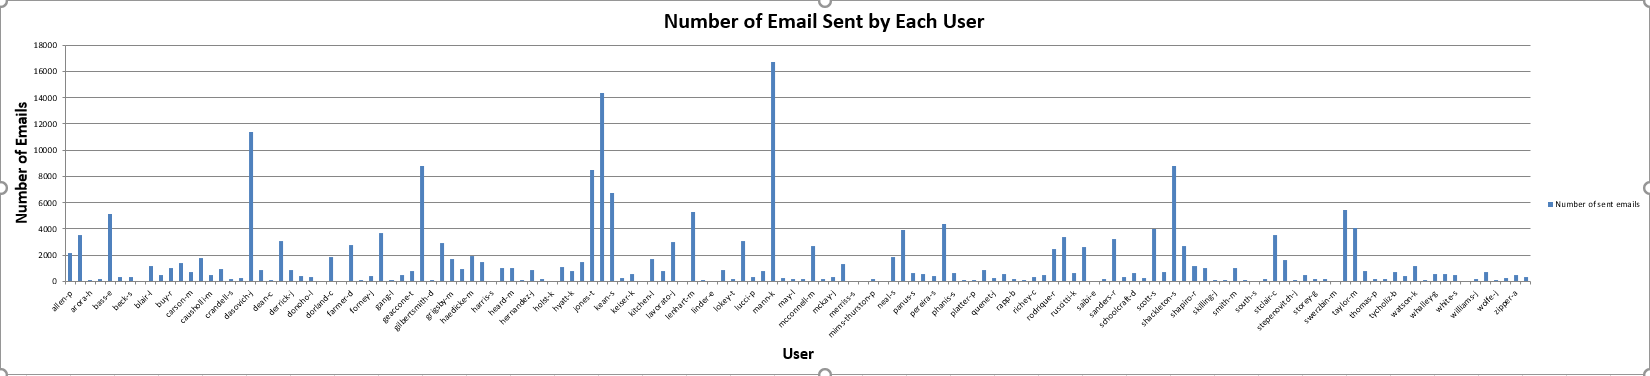
\includegraphics[width=\textwidth]{emails_sent.png}
			\caption{Number of emails sent per user.}
			\label{fig:emails_sent}
		\end{figure}
		
		\begin{figure}[h]
			\centering
			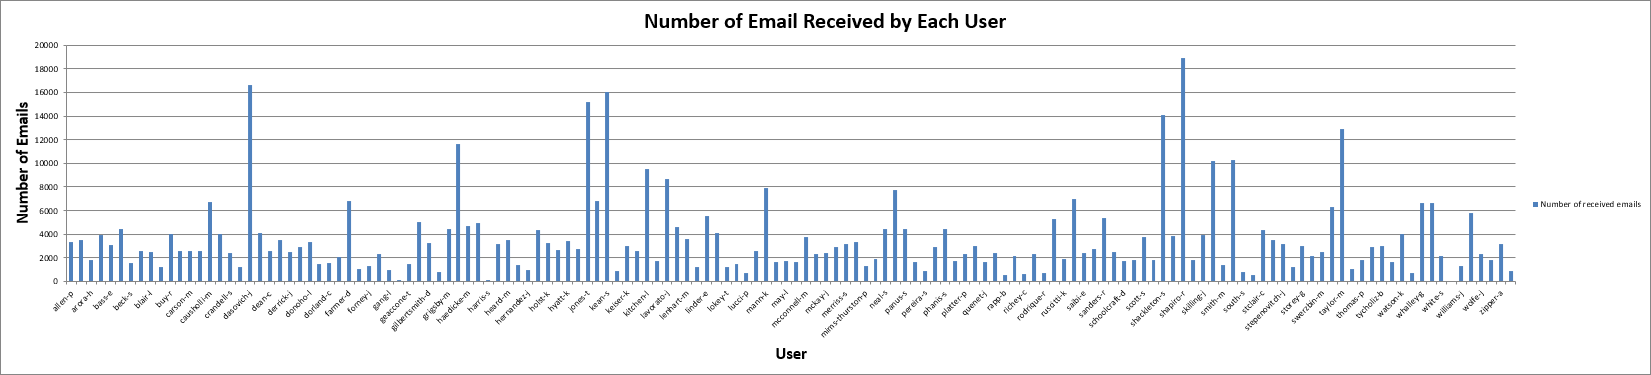
\includegraphics[width=\textwidth]{emails_received.png}
			\caption{Number of emails received per user.}
			\label{fig:emails_received}
		\end{figure}
		
		\begin{figure}[h]
			\centering
			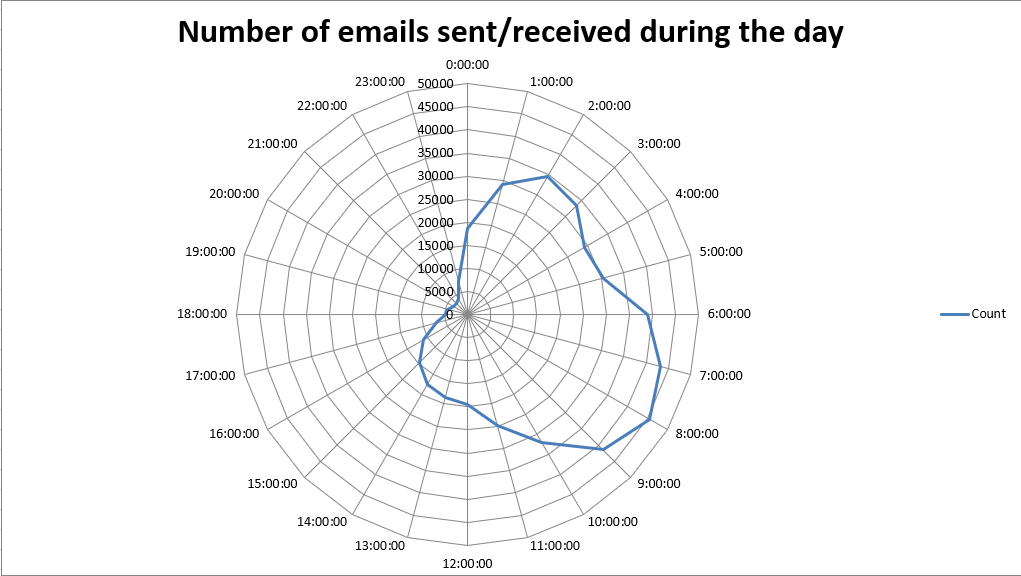
\includegraphics[width=\textwidth]{time_sent.png}
			\caption{Time of the day emails were sent/received.}
			\label{fig:time_sent}
		\end{figure}
		
		\begin{figure}[h]
			\centering
			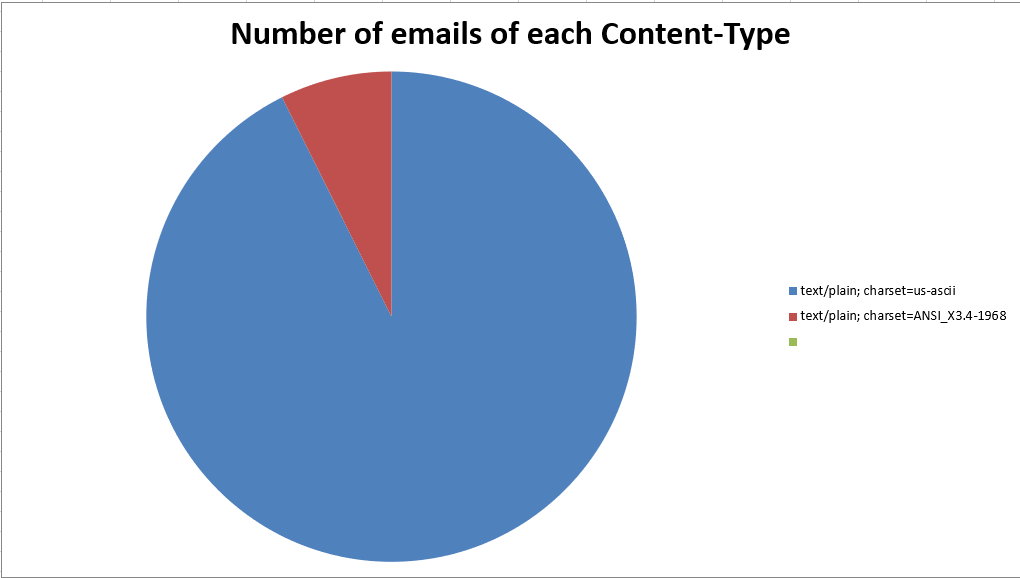
\includegraphics[width=0.6\textwidth]{content_type.png}
			\caption{Content type used in emails.}
			\label{fig:content_type}
		\end{figure}
		
		\begin{figure}[h]
			\centering
			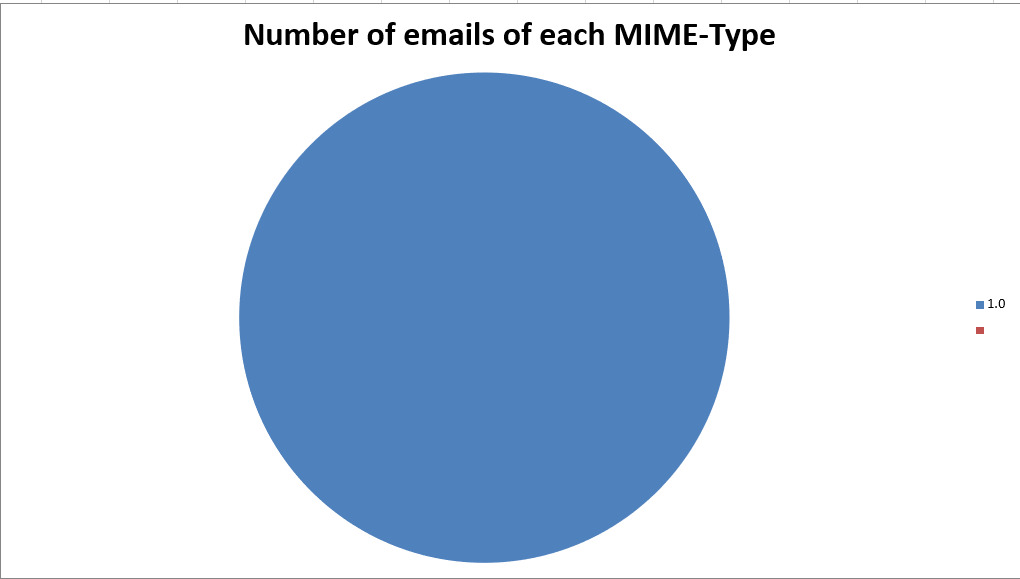
\includegraphics[width=0.6\textwidth]{mime_type.png}
			\caption{MIME type used in emails.}
			\label{fig:mime_type}
		\end{figure}
		
		\begin{figure}[h]
			\centering
			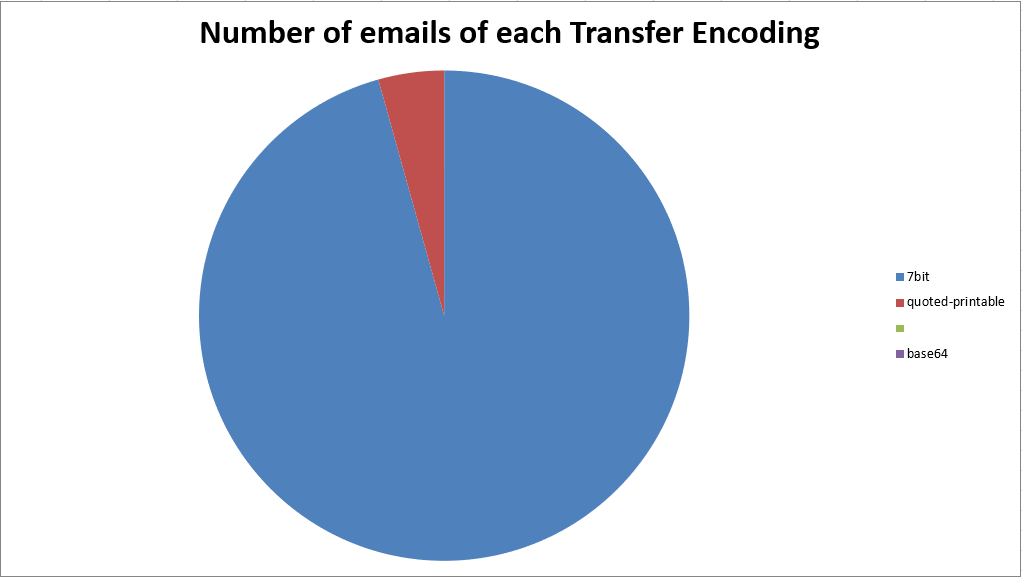
\includegraphics[width=0.6\textwidth]{transfer_encoding.png}
			\caption{Transfer encoding used in emails.}
			\label{fig:transfer_encoding}
		\end{figure}
		
		\begin{figure}[h]
			\centering
			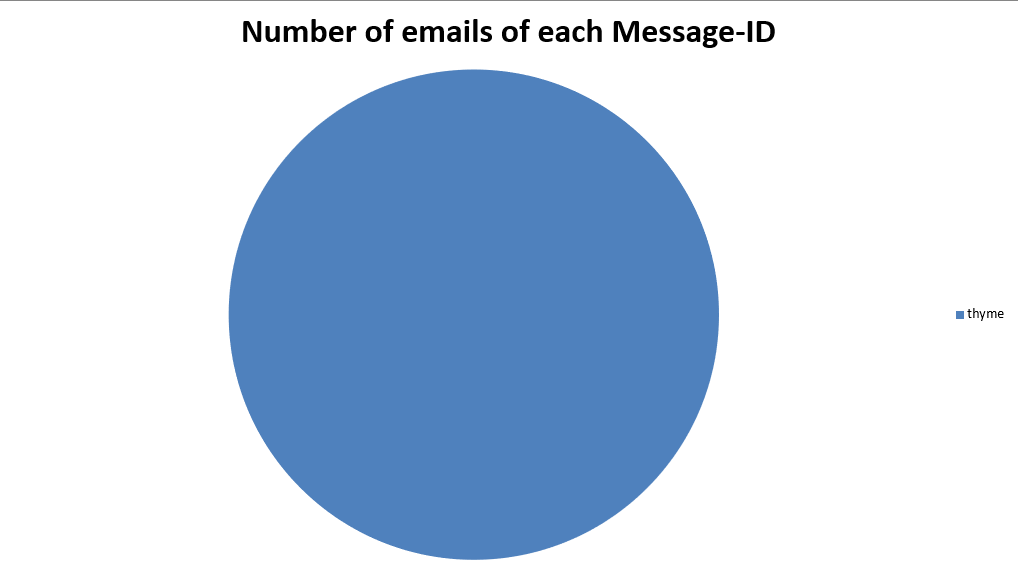
\includegraphics[width=0.6\textwidth]{message_id.png}
			\caption{Message ID domain used in the emails.}
			\label{fig:message_id}
		\end{figure}
		
		\begin{figure}[h]
			\centering
			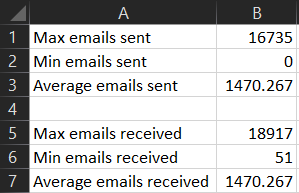
\includegraphics[width=0.6\textwidth]{descriptive_statistics.png}
			\caption{Descriptive statistics on sent/received emails.}
			\label{fig:descriptive_statistics}
		\end{figure}
 
		
	\section{Attribute Identification}
		\paragraph\indent
            After analyzing the results from the EDA phase and a more in-depth understanding of the ``landscape'' of the data was obtained we performed attribute identification. This involved picking certain attributes that could (after some potential remodeling) be used by the machine learning tools to be able to more accurately classify the data.\\
        
        The following attributes of the headers were identified, which would potentially aid in detecting abnormal or malicious emails. \cite{Karlapalem2017} \cite{Faulkner2016} 
        
        \begin{itemize}
					\item Received1\\
							Can be used to identify if the receiving server has a malicious IP address by using a predefined list of malicious blacklisted IP addresses.
					\item Received2\\
							Can be used to identify if the sending server has a malicious IP address by using a predefined list of malicious blacklisted IP addresses.
					\item Message-ID\\
							In the Enron emails the domain of the message ID do not match the sender's email address domain. It is suspected that this was changed during the clean up of previous research since the two usually matches. Therefore, we did not utilize this technique ad only focuses on whether the domain specified is malicious or not.
					\item From\\
							The from field will be used to check if it is in anyway suspicious, or has any obvious indicators of a fabrication. An example of this would be a domain in the email address that is similar to a legitimate domain, like ``claims@netbank.co.za'' instead of ``claims@nedbank.co.za''. Unfortunately, due to time constraints this was omitted from our tests.
					\item To\\
							Mass spam and malicious emails often contain a large amount of recipients. This field can thus be used to check the number of addresses in the "To" field.
					\item Subject\\
						The Subject can be used to detect phishing emails based on the presence of certain characteristics, like the presence of special characters. 
					\item X-To\\
						The X-To field can be used similar to the To field, to check how many other recipients there are to that email.
					\item X-cc\\
						The X-cc field can be used similar to the To field, to check how many other recipients there are to that email.
					\item X-bcc\\
						The X-bcc field can be used similar to the To field, to check how many other recipients there are to that email.
					\item Cc\\
							The Cc field can be used similar to the To field, to check how many other recipients there are to that email.
					\item Bcc\\
							The Bcc field can be used similar to the To field, to check how many other recipients there are to that email.
				\end{itemize}
		
		
	\section{Feature Engineering}
		\paragraph\indent
		Feature Engineering was done by using the attributes identified above and processing them into values that can be interpretable for machine learning, as well as useful in detecting possible malicious emails.\cite{Karlapalem2017} \cite{Faulkner2016} \cite{Al-jarrah2012}
        
        \begin{itemize}
					\item To\\
							This gives the number of ``To'' contacts in the email.
					\item X-To\\
							This gives the number of ``X-To'' contacts in the email.
					\item X-cc\\
							This gives the number of ``X-cc'' contacts in the email.
					\item X-bcc\\
							This gives the number of ``X-bcc'' contacts in the email.
					\item Cc\\
							This gives the number of ``Cc'' contacts in the email.
					\item Bcc\\
							This field gives the number of ``Bcc'' contacts in the email.
					\item Possibly-Spam-Subject\\
						The Possibly-Spam-Subject is set to true if the subject is found to have characteristics of Spam mail.
					\item Bcc-Larger-Than-CC\\
						This field is a boolean value which is set to true if the number Bcc contacts is larger than the contacts found in the CC field. Otherwise it's set to false.
					\item Bcc-Larger-Than-To\\
						This field is a boolean value which is set to true if the number Bcc contacts is larger than the contacts found in the To field. Otherwise it's set to false.
					\item Blacklisted-IP-Address\\
							The Blacklisted-IP-Address field is a boolean which is set to true if the IP addresses found in the Received fields or in the From-IP field, matches an IP address in the blacklist of known servers found to be used for malicious emails.
                    \item Special-Chars-Subject\\
                    		The Special-Chars-Subject is a count of special characters such as ``\$' and ``!' in the subject line.
                    \item Count-Uppercase-Chars-Subject\\
                    		The Count-Uppercase-Chars-Subject is a count of how many characters are uppercase in the subject line.
                    \item Subject-Length\\
                    		The Subject-Length is the length of the subject line. Together with Count-Uppercase-Chars-Subject the subject line is checked to see if the entire subject line is capitalized.
				\end{itemize}
		
	\section{Using Machine Learning to Detect Abnormal Behavior}
		\paragraph\indent
		

		\subsection{Decision tree}
			\indent\subsubsection{Setup}
			\paragraph\indent
            The following was done to prepare the machine learning system.
            \begin{itemize}
              \item Create training dataset\\
              \begin{itemize}
                    \item A training dataset with a size of 74 entries was created. 
                    \item The training dataset consists of non-malicious emails,as well as malicious emails of various nature. 
                    \item The training dataset is based findings from the feature engineering section, and has an additional boolean field named 'Possibly-Malicious', which is used as the target value for the training set.
              \end{itemize}  
              \item Create full dataset\\
              \begin{itemize}
                    \item A dataset containing the data of all the emails was created to test the accuracy of the model.
                    \end{itemize}
            \end{itemize}
            \indent\subsubsection{Results and interpretation}
            \begin{figure}[h]
              \centering
              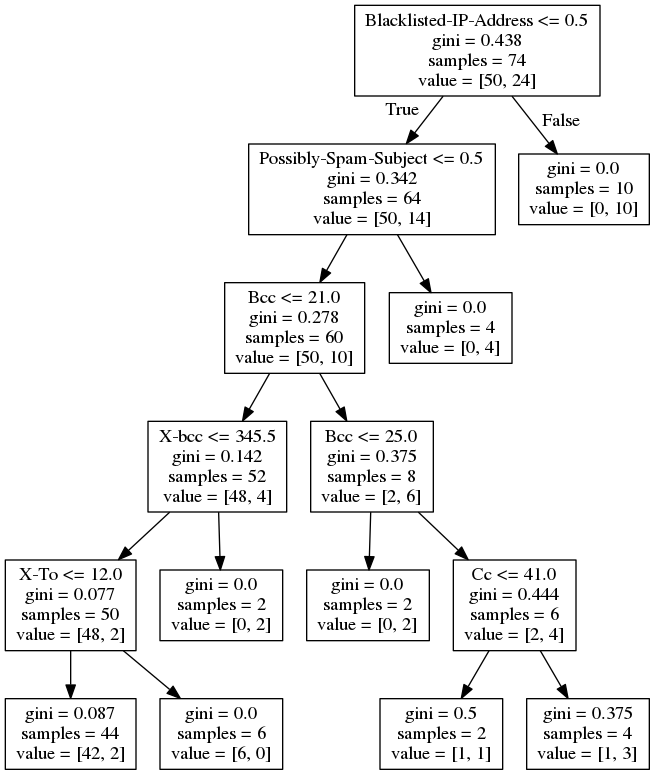
\includegraphics[width=0.6\textwidth]{decision_tree_model.png}
              \caption{The decision tree model that was generated using the training dataset}
              \label{fig:decision_tree_model}
			\end{figure}
			\paragraph\indent
            \begin{itemize}
              \item Interpreting the model\\
              Figure \ref{fig:decision_tree_model} shows the decision tree model which was generated from the training dataset.
              Interpreting the model shows us that if Blacklisted-IP-Address is found to be true (>0.5), then the email will be found to be malicious. However, if it is found to be false (<=0.5) it will check the value of Possibly-Spam-Subject. If Possibly-Spam-Subject is true, then emails may also be found malicious. However if it's found to be false, then it moves to the next criteria, by check the values of Bcc. If the value was <=21 then the X-bcc and X-To will be checked. If it was >21 then the Bcc will be checked again as well as the Cc.
            \end{itemize}
            \begin{itemize}
              \item Accuracy results on the full dataset\\
            	The accuracy yielded after running a prediction on the full dataset was 99.6\%. This is an indication that the model generated from the learning dataset is a good prediction on malicious emails in the full dataset. 
            \end{itemize}
            
            
		\subsection{Comparing rule induction and Naive Bayes}
			\paragraph\indent
			 RapidMiner was used to setup a performance measure between Rule Induction machine learning, Naive Bayes and Decision Tree. The Confusion matrix and ROC of both algorithms are compared.
            \indent\subsubsection{Setup}           
            \begin{itemize}
              \item The data is first preprocessed to get more reliable data\\
                  \begin{itemize}
                    \item First a subset of attributes are selected from the results of feature engineering
                    \item After that any rows with missing data is removed, this results in the dataset being reduced from 517 401 entries to  493 043 entries.
                  \end{itemize}
				\item The data is then sent to the machine learning algorithm and the performance is measured
                	\begin{itemize}
                		\item First the data is split in two with a ratio of 70\% and 30\%
                        \item The 70\% gets fed into the machine learning algorithm
                        \item The prediction column (Possibly-Spam-Subject) is removed from the 30\% dataset for validation
                        \item The validation dataset is applied to the resulting model from the machine learning algorithm and compared to the input dataset to measure the performance. Figure \ref{fig:rapidminer-model} is an example of how the model looks like in RapidMiner.
                	\end{itemize}
            \end{itemize}
            \begin{figure}[h]
            	\centering
                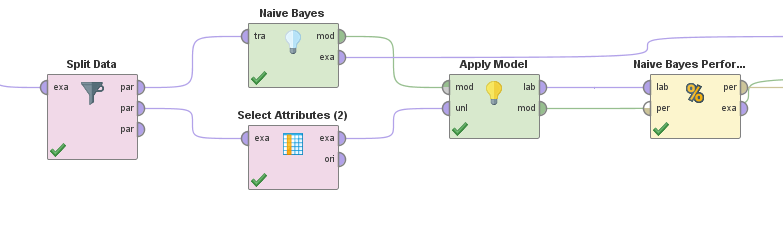
\includegraphics[width=\textwidth]{Model.PNG}
                \caption{The resulting model in RapidMiner for one of the algorithms}
                \label{fig:rapidminer-model}
            \end{figure}
            
    	\subsubsection{Results and interpretation}
        The overall accuracy for rule induction is 96.2\% and Naive Bayes is 99.64\%. Thus far it looks like Naive Bayes is the better algorithm to use between Rule Induction and Naive Bayes. Further investigation is done to prove the previous statement.
        
        Looking at the ROC curve between the algorithms in figure \ref{fig:roc} we can see that Rule Induction jumped straight to the top left corner. This indicates that Rule Induction only predicted one outcome for all emails. It seems that Rule Induction did not correctly classify malicious emails. Upon further investigation we look at the confusion matrix for Rule Induction.
        \begin{figure}[h]
        	\centering
            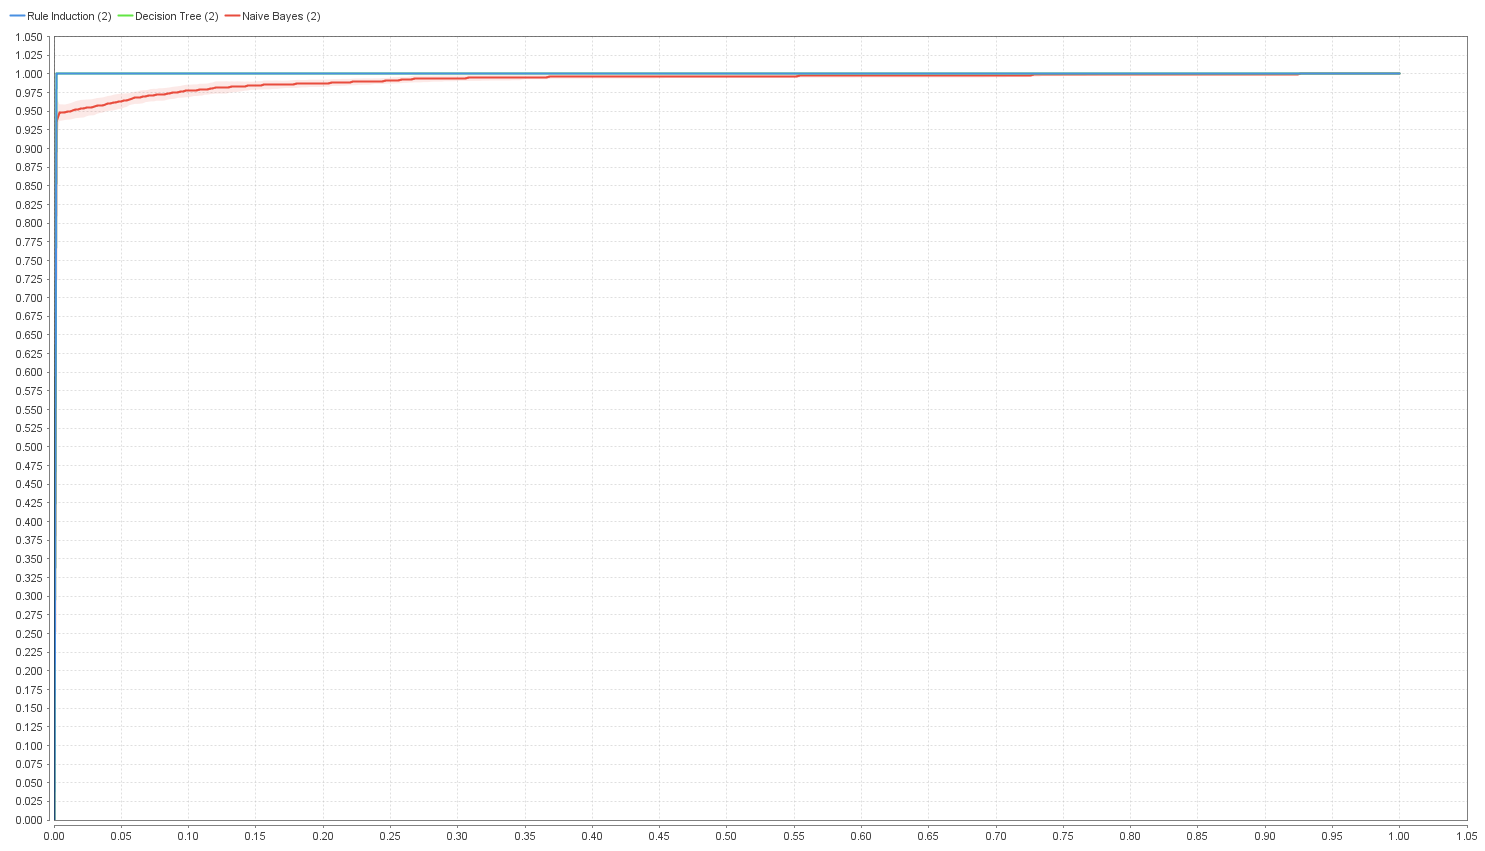
\includegraphics[width=\textwidth]{ROC.PNG}
            \caption{ROC graph comparing the algorithms}
            \label{fig:roc}
        \end{figure}
        
        Looking at the confusion matrix of rule induction in figure \ref{fig:rule-induction} the class recall is 100\% for actual value ``false'' yet the algorithm only achieved 96.2\% prediction rate for value ``false'', and the algorithm did not predict true at all. We suspect that the algorithm split the data up in such a way that the validation set had no fields to predict true, or that the algorithm was not suitable to predict malicious emails correctly.
        \begin{figure}[h]
        	\centering
            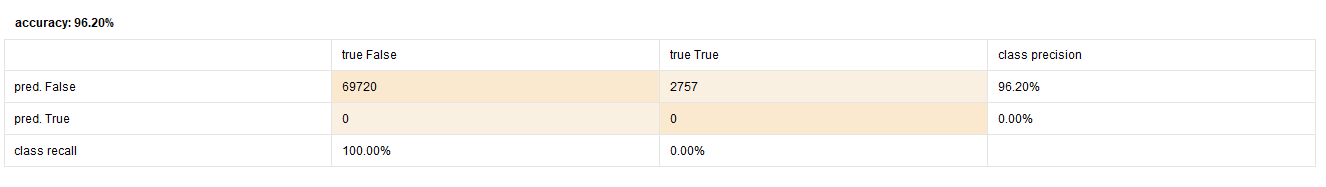
\includegraphics[width=\textwidth]{Rule-induction-cunfusion-matrix.PNG}
            \caption{Rule induction confusion matrix}
            \label{fig:rule-induction}
        \end{figure}
        
        Comparing the ROC curve of Naive Bayes in figure \ref{fig:roc}, the curve for Naive Bayes algorithm looks more realistic. The confusion matrix for Naive Bayes in figure \ref{fig:naive-bayes} also has more realistic prediction accuracies of 99.7\% and 97.01\% for value ``false'' and ``true'' respectively. This may indicate that the selected attributes from the training data may have not stated clear enough rules for rule induction and resulted a bias towards false prediction, causing the rule induction operator to be very inaccurate.
        
        The results show that Naive Bayes has more realistic performance measures compared to Rule Induction. Therefore Naive Bayes may be more suitable for training on email header data. Compared to Decision tree it seems like decision tree has higher accuracy and therefore may be the best performing algorithm.
        \begin{figure}[h]
        	\centering
            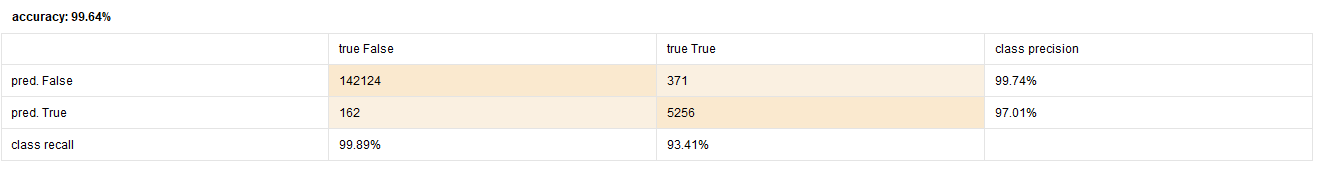
\includegraphics[width=\textwidth]{Naive-bayes-confusion-matrix.PNG}
            \caption{Naive Bayes confusion matrix}
            \label{fig:naive-bayes}
        \end{figure}               
            
	\section{Cyber Criminal Profiling}
		\paragraph\indent
		The machine learning models generated above, assisted in creating various cyber criminal profiles.
        \begin{itemize}
        	\item Profile A
            \begin{itemize}
        		\item This criminal uses an email server with an IP-address that is blacklisted and was immediately detected.
        	\end{itemize} 
            \item Profile B
            \begin{itemize}
        		\item This criminal was not detected using an email server with an IP-address that is blacklisted.
                \item However the Subject header was detected as a possible spam-subject.
        	\end{itemize} 
            \item Profile C
            \begin{itemize}
        		\item This criminal was not detected using an email server with an IP-address that is blacklisted.
                \item The Criminal's Subject line was not picked up as a spam-subject.
                \item The Criminal sends the email to a large number of recipients in Bcc, Cc and To fields. 
        	\end{itemize} 
        \end{itemize}
        The differing Profiles indicate that there could be a difference in experience from one cyber criminal to another. With some criminals more experience and able to cover their tracks, or their targets being easier to convince.\cite{Bada2016}
		
	\section{Anonymization}
		\paragraph\indent
        The following steps were followed in order to anonymize the email databset:
        \begin{itemize}
        	\item The process of anonymization starts with removing the email body in an attempt to reduce the chances of personal information leaked that may be contained in an email body.
            \item Thereafter any 6 to 16 digit numbers in the subject line are masked as ten 0's (0000000000).
            \item The account part in all the email addresses are hashed using the MD5 hashing algorithm. The reason for hashing the account part of the email addresses is to keep all masked email addresses the same to facilitate cross matching. The domain part of each email is kept as is to facilitate comparing the emails to known malicious email addresses.
            \item Any extra strings in the X-headers are also hashed as they may contain the full name of the owners of their respective email addresses. This is to protect the identities of the owners of each email address.
            \item Additional processing is done to put all email lists inline instead of having each email address in a list on it's own line. This is done for easier processing later on.
            \item The anonymized emails are saved to another folder after they have been anonymized.
        \end{itemize}         
		
		
	\bibliographystyle{unsrt}
	\bibliography{bibliography}
\end{document}